%%%%%%%%%%%%%%%%%%%%%%%%%%%%%%%%%%%%%%%%%%%%%%%%%
% Relatório Final - Projeto de Pesquisa
% Métodos de Otimização
% Baltz & Machado
% Capítulo 2
%%%%%%%%%%%%%%%%%%%%%%%%%%%%%%%%%%%%%%%%%%%%%%%%%


\chapter{\Large{Métodos Clássicos de Otimização}}\label{chp:2}


\section{{O Método de Newton}}


\subsection{Entendendo o Método}

%TODO: Falar de funções bem definidas

\hspace{0.8cm}
O Método de Newton, foi desenvolvido com o objetivo de econtrar estimativas
para as raízes de uma função. De modo que, a execução do método é feita de
forma iterativa, repetindo sempre o mesmo processo, atualizando o mesmo valor.

Este método faz uso do recurso de derivação, existindo, uma relação muito
forte com o ângulo da reta tangente ao ponto, na função. Ademais, é
importante ressaltar, que é necessário um palpite inicial, que represente
o valor de \textit{x}, no qual, partindo desse valor, será buscado a raiz.
E com isso, vamos entender como o dado método funciona.

Partindo do princípio do método, o objetivo, será utilizar a reta tangente a um
ponto, para gerar valores cada vez mais próximos da raiz daquela função. De
modo que, será analisado a interseção da reta tangente com o eixo das
abscissas. E sendo, a diferença do valor x da entrada da função com o valor da
fração entre a função e sua derivada no mesmo ponto, o novo valor de entrada na
função, construindo assim várias iterações, gerando valores cada vez mais
próximos da raiz. Como será visto, a seguir:

Já sabido que a equação da reta é dada como:

\begin{equation}
    (y - y_0) = m(x - x_0).
\end{equation}

E levando em conta que temos como objetivo encontrar $x$, que é um ponto
sobreposto no eixo x, podemos considerar $y=0$, logo:

\begin{equation}
    -y_0=m(x-x_0).
\end{equation}

Com isso, sabemos que $y_0$ é a imagem da função $f(x_0)$, e $m$ representa o
ângulo da reta tangente ao ponto $x_0$, ou seja: $m=f'(x_0)$. Desenvolvendo
essa equação, temos:

\begin{equation}
    -f(x_0) = f'(x_0)(x-x_0),
\end{equation}

\begin{equation}
    -f(x_0) = f'(x_0)x - f'(x_0)x_0,
\end{equation}

\begin{equation}
    0 = f'(x_0)x - f'(x_0)x_0+f(x_0),
\end{equation}

\begin{equation}
    0 = x - x_0 + \frac{f(x_0)}{f'(x_0)},
\end{equation}

\begin{equation}
    x = x_0 - \frac {f(x_0)}{f'(x_0)}.
\end{equation}\\

E com isso, exemplificando em um gráfico, temos que, sendo $f(x)=-x^2+2x$, o
palpite inicial $x_0=1.5$, $P1$ sendo o ponto que representa $x_0$ aplicado
a função $f$ e $x1$ a interseção da reta tangente à $P1$ com o eixo x.

\begin{figure}[ht]
    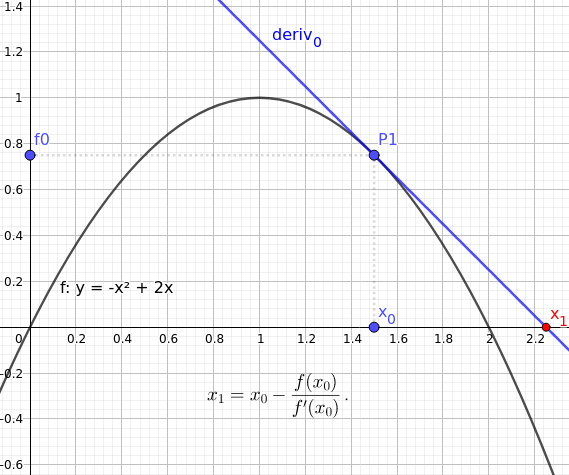
\includegraphics[width=0.55\textwidth]
      {src/MetodoNewton_grafico_1.png}
    \centering
    \caption{
      Primeira iteração do Método de Newton.
     }
    \label{MetodoNewton_grafico_1}
\end{figure}


E a partir do dado gráfico, agora podemos entender melhor como a iteração
funcionará, pois, o valor gerado, $x_1$, será aplicado no mesmo método. E com
isso, podemos construir a seguinte equação:

\begin{equation}
    x_{k+1} = x_{k} - \frac {f(x_{k})}{f'(x_{k})}.
    \label{newton_primeiraDeriv}
\end{equation}

Desse modo, gera-se uma sequência $\{x_k\}$, donde, esta, converge para a
raiz da função. E nesse sentido, vejamos a próxima iteração (Figura
\ref{MetodoNewton_grafico_2}) do exemplo mostrado na Figura
\ref{MetodoNewton_grafico_1}.

\begin{figure}[ht]
    \centering
    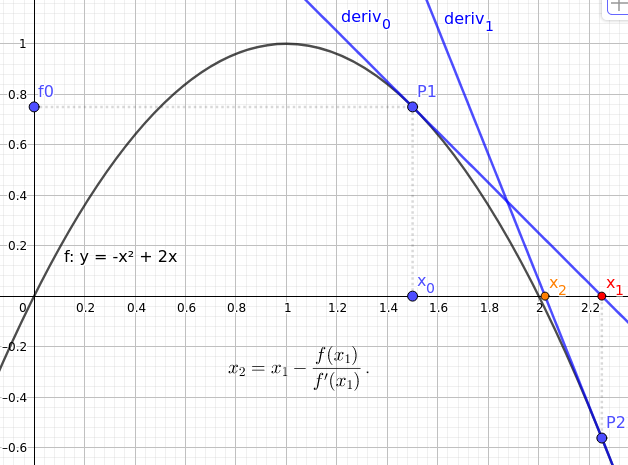
\includegraphics[width=0.55\textwidth]
      {src/MetodoNewton_grafico_2.png}
    \caption{
      Segunda iteração do Método de Newton.
    }
    \label{MetodoNewton_grafico_2}
\end{figure}

E assim, podemos notar a aproximação de $x_k$ para a raiz de $f$, observando o
ponto $x_2$.

Ademais, é válido ressaltar que o denominador da equação
\ref{newton_primeiraDeriv} tem que ser diferente de 0 (ou seja, a reta tangante
num ponto $P$ não pode ser paralela ao eixo x). No entanto, caso contrário,
isso significa que a dada função não possui raiz na proximidade daquele ponto.

\subsection{Encontrando Mínimos}

E é dessa maneira que, agora, podemos utilizar este método para encontrar
mínimos de uma função. Vimos que, o Método de Newton calcula raízes, e
desse modo, vinculando o que foi estudado no Capítulo 1, sabemos que, os
mínimos de uma função podem ser representados como raízes de sua derivada.

%TODO: Falar mais/melhor sobre a sequencia {x_k} (tendencia ao 0 da função)

Então, dado que as raízes de $f(x)$ podem ser geradas a partir da equação
\ref{newton_primeiraDeriv}, temos que: considerando $g(x)$ uma função duas vezes
derivável, e tendo como objetivo encontrar seus pontos de mínimo, pode-se
utilizar o Método de Newton para resolver tal problema da seguinte forma:

\begin{equation}
    x_{k+1} = x_{k} - \frac {g'(x_{k})}{g''(x_{k})}.
\end{equation}

Encontrando então as raízes aproximadas de sua derivada, e considerando
estas como  $x^*$, temos então que:

\begin{equation}
    g'(x^*) = 0.
\end{equation}

O método é simples, entrega muitas vezes ótimos locais próximos ao ponto
inicial, mas tem seu destaque, que é ser, facilmente computável.

Problemas de maximização podem ser vistos sob o seguinte olhar:

\begin{equation}
    max(f(x)) = min(-1 * f(x))
\end{equation}

Que com isto podem ser otimizados pelo Método de Newton também.

O movimento de \(x_k\) dentro da sequência, é determinado pela relação das
quantidades e propriedades, que tanto a primeira quanto a segunda derivada
oferecem. As quantidades, determinam a velocidade do movimento, e os sinais,
indicam a direção do movimento. De certa forma, podemos interpretar o movimento
da sequência \(\{x_k\}\) como instantes do movimento de uma bola numa ladeira,
que no começo de sua descida é acelerada, e, conforme chega ao plano no fim da
ladeira, começa a reduzir sua velocidade, até supostamente chegar no ponto mais
baixo.


\section{{Outros Métodos}}

Com o advento do Método de Newton, acabou surgindo uma família de métodos
similares. E como foi visto, é possível a partir dele, encontrar tanto raízes
de funções, quanto máximos/mínimos, herdando essa características para vários
dos métodos que o derivaram. São estes, chamados de Métodos Quasi-Newton,
que, olhando como ponto de partida o Método de Newton, fornecem uma grande
flexibilidade em como deseja-se utilizar os recursos de presição e poder
computacional.

Ademais, vejamos alguns outros métodos de otimização:

\subsection{Método do Gradiente Descendente}

Este, classificado como um Método Quasi-Newton, resolve os mesmos tipos de
problemas que os do método herdado. Considerando que o Método de Newton
encontra o \(min(f(x))\) através de uma sequência \(\{x_k\}\):

\begin{equation}
    x_{k+1} = x_{k} - \frac {f'(x_{k})}{f''(x_{k})}.
\end{equation}

No qual, pode ser reescrito da seguinte forma:

\begin{equation}
    x_{k+1} = x_{k} -  \frac{1}{f''(x)} * f'(x_{k}).
\end{equation}

E, ressaltando que, sabemos que quem determina a direção da convergência é
\(f'(x)\), não é completamente necessário o uso de \( \frac{1}{f''(x)} \), que
tem como principal papel de controlar o tamanho do `passo dado' na iteração.
De modo que, a maioria dos Métodos Quasi-Newton fazem a substituição
da dada fração por aproximações boas o suficiente. E com isso, levando em
conta $\alpha$ como a representação dessa aproximação, temos:

\begin{equation}
    x_{k+1} = x_{k} -  \alpha * f'(x_{k}).
    \label{newton_lambda}
\end{equation}

Onde \(\alpha\) satisfaz:

\begin{equation}
    f(x_{k} -  \alpha * f'(x_{k})) < f(x_{x}).
    \label{newton_restricao_alpha}
\end{equation}

A partir da equação \ref{newton_lambda}, podemos escolher um \(\alpha\), de
modo que, seja menos custoso encontrá-lo do que calcular a segunda derivada
da função objetivo, ou até, podemos nem calculá-lo, basta considerar
um \(\alpha\) fixo, e tão pequeno que, quando a restrição
\ref{newton_restricao_alpha} não for cumprida, temos uma aproximação boa o
suficiente para o minimo da função.


\subsection{Simplex}

\hspace{0.8cm}
O método Simplex, pode ser classificado como clássico, por ser um
dos métodos mais famosos. Formulado por George B. Dantzig, fruto de uma
sugestão de outro homem, T. S. Motzkin, que contribuiu para diversas áreas da
matemática.

Os problemas que o método Simplex resolve, fazem parte de uma conjunto de
problemas de Otimização Linear (ou Programação Linear), os quais se restringem
a, apenas, funções lineares. Além disso, tais problemas normalmente acompanham
restrições, sobre as entradas da função a ser otimizada.

Um problema de otimização linear, pode ser resumido em:

\begin{equation}
        Z = c_1x_1 + c_2x_2 + … + c_nx_n
\end{equation}

E tendo restrições também lineares para a função objetivo, como:
\begin{equation}
    \begin{split}
        &   a_{11}x_1 + a_{12}x_2 + … + a_{1n}x_n \leq b_1\\
        &   a_{21}x_1 + a_{22}x_2 + … + a_{2n}x_n \leq b_2\\
        &   ...\\
        &   a_{m1}x_1 + a_{m2}x_2 + … + a_{mn}x_n \leq b_m\\
        &   x_1 \geq 0, x_2 \geq 0, …, x_n \geq 0
    \end{split}
\end{equation}

O tipo de problema que o Simplex resolve, se desenvolve como a seguir:

\begin{equation}
        max \{c^tx | Ax \leq b, x \geq 0\}\\
\end{equation}


A forma de operação desse método é semelhante ao que uma pessoa comumente faria
ao se deparasse com o problema de forma gráfica. O problema, sendo
completamente linear, gera retas, que acabam por formando regiões de
possíveis soluções, e dessas regiões, queremos saber qual a melhor solução.
Para isso, bastaria procurar dentro de tal região, onde o valor da função Z é o
maior possível. Uma vez a região sendo construída por retas, acaba por
ter a característica de ser convexa, como um polígono convexo no plano ou um
poliedro convexo no espaço, o que a acaba por facilitar a busca pelo máximo,
dentro dessa região, uma vez que basta olha os vértices de tal região.

Repara-se, que, o método Simplex não se utiliza de artifícios e ferramentas do
Cálculo, como nos métodos anteriormente apresentados, mas sim, formas
diferentes de analisar o problema, que por certos aspectos é simples. O método
completo é constituído por operações em uma matriz específica (Tableau), que
representa o problema, o qual não é necessário ser apresentado aqui, por se
distanciar da `família' de métodos de otimização que é apresentado neste
documento.



\section{{Programando os Métodos}}

\hspace{0.8cm}

\subsection{Método de Newton}

\hspace{0.8cm}
A forma mais simples e mais útil de implementar o Método de Newton, é na forma
de busca das raízes, que, uma vez implementada, só precisamos por como entrada
a primeira e a segunda derivada da função que desejamos minimizar, já que o
método não precisa saber qual a função de fato. A seguir temos a implementação
na linguagem de programação \textit{Rust}:
\vspace{0.2cm}
\begin{lstlisting}
pub fn newton1x1<F>(funcao_derivada: &F, x: f64) -> (usize, f64)
where
    F: Fn(f64) -> f64,
{
    let mut entrada_atual = x;
    let maximo_iteracoes = 100;

    for iteracao_atual in 1..=maximo_iteracoes {
        let diferenca: f64 =
            funcao_derivada(entrada_atual.clone())
            /
            derive1x1(&funcao_derivada, &entrada_atual);

        println!("diferenca: {}", diferenca);
        entrada_atual -= diferenca;

        if diferenca.abs() < 0.0000001 {
            return (iteracao_atual, entrada_atual);
        }
    }

    return (maximo_iteracoes, entrada_atual);
}
\end{lstlisting}


Os parâmetros da função são:

    \begin{itemize}
            \item Uma função \(f : \mathbb{R} \rightarrow \mathbb{R}\)
            \item Uma entrada x sendo o chute inicial do ótimo.
    \end{itemize}


A função \textit{derive1x1}, recebe como parâmetro uma função e um ponto,
tendo como retorno, a derivada da função entregue, no ponto especificado.
Restringindo-se à funções do tipo \(f : \mathbb{R} \rightarrow \mathbb{R}\).


\subsection{Método do Gradiente Descendente}

\hspace{0.8cm}
A implementação desse método, exige apenas, que seja definido o cálculo
da derivada da função objetivo, o valor de $\alpha$, um palpite inicial para
o valor de x, e a quantidade de iterações desejada. Também, pode ser
indicado um valor que se refere a diferença dos dois últimos valores
da sequência \{$x_k$\}, podendo assim, efetuar a parada da execução do
método. A seguir, temos a implementação na linguagem de programação
\textit{C++}:

\vspace{0.2cm}
\begin{lstlisting}[language=C++]

// Sendo f(x) = x^4 - 3*x^3 + 2
#include <bits/stdc++.h>
#define decimal long double
using namespace std;
// Calcula a derivada da funcao
decimal df(decimal x) {
	return 4 * pow(x, 3) - 9 * pow(x, 2);
}
int main() {
	// Palpite inicial
	decimal x_proximo = 5.5;
	// Variavel para iterar
	decimal x_atual;
	// Quantidade maxima de iteracoes
	int iteracoes = 100000;
	decimal alpha = 0.00001;
	// Precisao para condicao de parada
	decimal precisao = 0.000000001;
	// Comeca as iteracoes
	while(iteracoes > 0) {
		x_atual = x_proximo;
		x_proximo = x_atual - (alpha * df(x_atual));
		decimal precisao_atual = x_atual - x_proximo;
		// Se atingir a precisao desejada
		if(abs(precisao_atual) < precisao)
			break; // Para as iteracoes
		// Conclui uma iteracao
		iteracoes -= 1;
	}
	cout << ``x que minimiza f(x) = '' << x_proximo << endl;
	// Saida do algoritmo:
	// --> x que minimiza f(x) = 2.25
	return 0;
}


\end{lstlisting}





\textcolor[rgb]{1,0,0}{\section{{O Método de Newton para Várias Variáveis}}}
